\documentclass[thesis.tex]{subfiles}
\begin{document}

\chapter{Methods}

\section{Detectors}

\subsection{Scale invariance}

\section{Descriptors}

\subsection{SIFT}

Gradients of an image are often used to describe the region around interest points, since they describe the changes in intensities in the image plane.
The \emph{scale-invariant feature transform} (SIFT) descriptor
\cite{lowe2004distinctive} is the most popular descriptor based on this
approach. It works by dividing the image regions surrounding interest
points into square cells and constructing a histogram of gradient
orientations for the pixels in each cell. The interest points are detected
using a multi-scale DoG detector. By computing the gradient orientations
at detection scale, the descriptor becomes scale invariant. The descriptor
is also rotation invariant as the cell grid is rotated according to the
dominating gradient orientation. Finally the descriptor achieves illumination
invariance by normalizing the histograms. The SIFT descriptor uses a grid of
$4 \times 4$ cells each consisting of $4 \times 4$ pixels, with 8 histogram
bins for each cell. This results in a dimensionality of $4 \times 4 \times 8 =
128$.

\subsection{PCA-SIFT}

\emph{PCA-SIFT} \cite{ke2004pca} is also based on combining oriented gradients
within a region, but instead of dividing the feature into cell histograms
it uses principal component analysis (PCA) to reduce the dimensionality
of the combined gradients. It also uses a multi-scale DoG detector for
interest point detection as SIFT. When computing PCA we compute the most
significant orthogonal dimensions of a dataset. In order to obtain good
results a large and diverse dataset of images and their features is required.
PCA-SIFT describes a single patch of $41 \times 41$ pixels. When computing
the gradients it gives gradient dimensionality of $2\times39\times39 = 3042$,
which is reduced by PCA to 36 dimensions.

\subsection{GLOH}

The \emph{gradient location and orientation histogram} (GLOH) descriptor
\cite{mikolajczyk2005performance} is an extension of the SIFT descriptor.
It differs from the SIFT descriptor by making a log-polar grid of
cells instead of rectangular cells. Furthermore the dimensionality of
the descriptor is reduced using PCA (on 47,000 patches according to
\cite{mikolajczyk2005performance}). The log-polar grid is split into three
rings at radius 6, 11, and 15, of which each of the two outer-most rings are
divided into eight angular cells giving a total of 17 cell bins. The gradient
orientations are divided into 16 bins giving a histogram of $16 \times 17
= 272$ bins. This is reduced to 128 dimensions by using the 128 largest
eigenvectors from PCA on a training dataset.

\subsection{DAISY}

The \emph{DAISY} descriptor \cite{tola2008fast} is a descriptor originally
developed for dense wide-baseline matching, and it is therefore developed
to create a descriptor of each pixel in an image very efficiently. The
descriptor is created from Gaussian directional derivative convolutions of
the image in eight directions and at three different scales. The use of these
convolutions allows for fast computations of simple convolutions compared
to the slower binning and post-processing used in SIFT. The descriptor of
each point is a concatenation of the eight directional derivatives of 25
points located in a circular grid shown in a daisy formation as shown in
Figure ??\todo{add daisy figure reference}. This results in a descriptor of
$25 \times 8 = 200$ dimensions. Further refinements of the algorithm and
experiments with the actual layout of the daisy formation have been examined
in \cite{winder2009picking}, in which the DAISY descriptor is claimed to perform
better than SIFT when used on the image correspondence problem.

\subsection{HOG}

The \emph{Histograms of Oriented Gradient} (HOG) descriptor is another
alternative to SIFT proposed in \cite{dalal2005histograms} for pedestrian
detection. Contrary to SIFT which is computed individually at specified
interest points, the HOG descriptors are computed in a dense grid over a
detection window and each block descriptor is a part of a larger descriptor
usually trained using an SVM. The Gradients are first computed using simple
1D masks. Secondly magnitude and spatially weighted histograms of the
orientations (0-180$^{\circ}$) of the gradients are computed for spatial
regions named cells\todo{Add note about interpolation of votes}. The cells are
then grouped together into blocks of cells for normalization to accomodate
for local illumination changes. These blocks can either be rectangular with
rectangular cells (R-HOG), or circular using a log-polar partitioning as the
DAISY descriptor. The normalization is performed using either the L2-norm,
a clipped and re-normalized L2-norm, or the square root of the L1-norm for
best performance. HOG descriptors are able to work directly on RGB images
unlike the original SIFT descriptor. This is done by computing the gradients
for each colour channel and choosing the gradient with the highest magnitude
for each pixel. For R-HOG the optimal bin number is found to be 9, optimal
block size $3\times3$ cell blocks and optimal cell size $6\times6$ pixels
with block spacing 8.\todo{Should optimal parameters for C-HOG be mentioned?}
Furthermore parts models using the HOG descriptor have been developed
\cite{felzenszwalb2008discriminatively} in order to improve upon the accuracy
of object detection.

\subsection{BIF-columns}

Another approach to descriptor design is to use higher order differential
information.
We use the term \emph{local $k$-jet} to refer to a vector
consisting of differential information up to order $k$ at some point.

\emph{Stability based similarity measure} (SBSM) \cite{balmashnova2008novel} for
matching of higher order differential information descriptors
Crosier and Griffin \cite{crosier2010using} base their texture representation, which
is just a descriptor but used for textures, on the local $2$-jet. They
partition the jet space into 6 Basic Image Features (BIFs) and compute these
across a region of pixels at four different scales. The chosen BIFs are
distinct texture elements such as dark spots and bright lines. Rather than
computing the distribution of BIFs at each scale, the four BIFs at each point
are combined into a BIF-column, and a histogram over all $6^4 = 1296$ possible
BIF-columns is computed. The 1296-dimensional descriptors are used for texture
classification.

\subsection{Jet descriptor}

\cite{larsen2012jet} have had success using local 4-jets. Their
$\mathcal{J}_4$-grid2 descriptor is computed from local 4-jets at four points
spread out across a pixel region. A whitening process is used on the jet
coefficients to scale normalize and decorrelate the descriptors, allowing for
Euclidean distance as a distance measure. The descriptor was evaluated against
state of the art on the image correspondence problem and performed favourably,
despite the simplicity of the descriptor.

\subsection{Galaxy descriptor}

Another recent higher order descriptor is the galaxy descriptor by Pedersen
et al.\cite{pedersen2013shape}, which is used to predict star-formation
rate from galaxy texture. The descriptor consists of multi-scale histograms
of gradient orientation as well as shape index, which is a simple 1D
representation of second order differential information. The histograms are
computed over a single region at eight scale levels.

\section{Matching strategies}
\label{sec:matching_strategies}

Thresholding, best-thresholding, ratio-thresholding.

\section{Performance measures}
\label{sec:performance_measures}

ROC, AUC, recall, 1-precision
\emph{Stability based similarity measure} (SBSM) \cite{balmashnova2008novel} for matching of higher order differential information descriptors.


\section{Invariants and robustness}
When describing interest points and their local regions in real world images we experience a lot of transformations of the actual physical objects. We are however interested in being able to describe the interest point without any of these transformations applied, in which case we have a better chance of recognizing the interest point in other images. In this section we will go through a list of possible transformations that we wish for our descriptor to be invariant to.

\todo{Add comment to robustness}

\begin{table}
\centering
\begin{tabular}{@{}l|ll@{}}
%\toprule
Measure & Rotation & Illumination \\
\hline
$\Theta$ & $\Theta - \theta $ & $\Theta$ \\
$M$ & $M$ & $a M$ \\
$S$ & $S$ & $S$ \\
$C$ & $C$ & $a C$ \\
%\bottomrule
\end{tabular}
\caption{The transformation of various measures by rotation and illumination. The derivations are included in \cref{apx:image_transformations}}.
\end{table}

\subsection{Translation}
The first transformation that we describe is translation. Translation occurs when images are taken from different positions and hence the interest points are translated in the image plane. Translation invariance is often achieved by combining a descriptor with an interest point detector which tells the descriptor where the interest points are located spatially in the image. Another approach is to use a sliding window technique in which a detection window is moved around the image trying to find a suitable matching position as in \cite{felzenszwalb2008discriminatively}. Translation invariance is almost always desired.

\todo{Add something about robustness against small translation errors}

\subsection{Rotation}
Rotation naturally occurs when either the camera or the object in question is rotated. Like the translation invariance we often get rotation invariance by combining the descriptor with an interest points detector. The detector often estimates the direction of the interest point based on the direction of the gradient in the interest point, and hence it outputs both translation and rotation invariant points to compute descriptors for. Rotation invariance is often desired but not always needed, as in \cite{dalal2005histograms,felzenszwalb2008discriminatively} where only detection of pedestrians in upright positions is needed. More general descriptors such as SIFT are however rotational invariant.

Refer to \cref{apx:rotation} for all rotations, \cref{apx:rotation_go,apx:rotation_m,apx:rotation_si,apx:rotation_c} for gradient orientation, gradient magnitude, shape index, and curvedness.
%
And thus $\widetilde{S}(x,y,\sigma) = S(x,y,\sigma)$.
%
\subsection{Reflection}

\subsection{Illumination}
Reference \Cref{apx:illumination} for $\Theta,~M,~S$, and $C$.
By using a small sigma for calculating the derivatives in the jet, we only use a small spatial area for the calculations which minimizes the risk of crossing a shadow edge. By combining multiple jets or shape indices into histograms we are able to calculate a descriptor across a shadow edge but still maintaining illumination invariance.

\subsection{Scale}
Noget med scalespace \cite{griffin1997scale}.

\subsection{Perspective}
noget med ?

\section{Calculating derivatives}
How to calculate n'th order n-dimensional derivatives of Gaussian.
No covariance in our equations (no skewed Gaussians)

\section{Histograms}

Histograms play an essential role in SIFT-like descriptors. They are used for aggregating gradient orientation (GO) and magnitude information over areas. Traditionally histograms have been constructed using hard boundaries between bins and with hard boundaries between the histograms of a descriptor such as \citet{lowe2004distinctive} does it in SIFT.\mycomment[MSN]{Should we explain SIFT's approach further?}

These types of histograms are however neither robust to small interest point translation/detection errors or gradient orientations close to the bin boundaries, and hence we here describe our histogram framework in which we are able to produce both ordinary as well as smooth histograms based on locally orderless images (LOI), \cite{koenderink1999structure}.

The idea behind smooth histograms is to remove the sharp boundaries of ordinary histograms and instead let all values contribute to all bins. The contribution of each value to each bin is dependent of the spatial distance to the cell center, the distance between the value and the bin center (angular distance for GO histograms) and the value weight (typically gradient magnitude for GO histograms).\todo{What about spatial weighting with respect to descriptor center as in SIFT}

Both of these distance weights are simple functions of a distance and hence we are able to compute ordinary histograms by using box functions and smooth histograms by using Gaussian functions.

NOTES:

Each bin is counted using a weighting function (bin filter) on all values centered in the bin with a width of $\sigma$.
Implemented so far: Gaussian, box, triangle

Renormalization to probability densities by computing the finite integrals of each bin which allows for varying bin sizes. See integral in section about Gaussian filter below.

Likewise possible to make histograms over periodic values (wrap-around over a defined interval).

Spatial weighting on each cell (magnitudes) possible as well as on the entire descriptor window.

Input variables when creating a histogram: inner scale $\sigma$, bin-width $\beta$, outer scale/size of ROI $\alpha$ according to \citet{koenderink1999structure}.



\subsection{Gaussian filter}

The 1-dimensional Gaussian filter with variance $\sigma$ is defined as:
%
\begin{align}
G(x;\sigma) = \frac{1}{\sqrt{2\pi} \sigma}
\exp\left( -\frac{x^2}{2 \sigma^2} \right)
\end{align}
%
The definite integral of $G(x;\sigma)$ from $a$ to $b$ cannot be expressed by an elementary function. Instead we can use the non-elementary error function, defined as $\mathrm{erf}(b) = \frac{2}{\sqrt{\pi}} \int_0^b \exp(-x^2) \,\mathrm dx$, which can be computed by its Taylor series. First we show an intermediate result using the substitution $u = \sqrt{k} x$ with $\mathrm du = \sqrt{k} \mathrm dx$:
%
\begin{align}
\int_0^b \exp(-k x^2) \,\mathrm dx
&= \frac{1}{\sqrt{k}} \int_0^{\sqrt{k}b} \exp(-u^2) \,\mathrm du \\
&= \frac{1}{\sqrt{k}} \frac{\sqrt{\pi}}{2} \mathrm{erf} \left( \sqrt{k} b \right)
\end{align}
%
We use this to compute $\int_a^b G(x;\sigma) \,\mathrm dx$:
%
\begin{align}
\int_a^b G(x;\sigma) \,\mathrm dx
&= \frac{1}{\sqrt{2\pi} \sigma} \int_a^b \exp\left( -\frac{x^2}{2 \sigma^2} \right) \,\mathrm dx \\
&= \frac{1}{\sqrt{2\pi} \sigma} \left( \int_0^b \exp\left( -\frac{x^2}{2 \sigma^2} \right) \,\mathrm dx - \int_0^a \exp\left( -\frac{x^2}{2 \sigma^2} \right) \,\mathrm dx \right) \\
&= \frac{1}{\sqrt{2\pi} \sigma} \frac{\sqrt{\pi}}{2} \sqrt{2} \sigma \left(
\mathrm{erf} \left( \frac{1}{\sqrt{2} \sigma} b \right) -
\mathrm{erf} \left( \frac{1}{\sqrt{2} \sigma} a \right) \right) \\
&= \frac{1}{2} \left(
\mathrm{erf} \left( \frac{b}{\sqrt{2} \sigma} \right) -
\mathrm{erf} \left( \frac{a}{\sqrt{2} \sigma} \right)
\right)
\end{align}
%
The $n$-dimensional Gaussian filter with variances $\boldsymbol{\sigma} = [\sigma_1, ..., \sigma_n]^T$ is defined as the product of $n$ 1-dimensional filters:
%
\begin{align}
G(\mathbf{x};\boldsymbol{\sigma})
&= \prod_i G(x_i;\sigma_i) \\
&= \frac{1}{(2\pi)^\frac{n}{2} \prod_i \mathbf{\sigma}_i}
\exp\left( -\sum_i \frac{x_i^2}{2 \sigma_i^2} \right)
\end{align}
%
With this definition we disallow arbitrary covariances as it does not make sense for a binning function. Note that the factors of $G(\mathbf{x};\boldsymbol{\sigma})$ contain distinct variables. Thus its definite integral from $a_i$ to $b_i$ in each dimension is simply the product of the definite integrals for each dimension:
%
\begin{align}
\int_{a_i}^{b_i} \dots \int_{a_n}^{b_n} G(\mathbf{x},\boldsymbol{\sigma}) \,\mathrm d{x_n} \dots d{x_i}
&= \prod_i \int_{a_i}^{b_i} G(\mathbf{x},\boldsymbol{\sigma}) \,\mathrm d{x_i} \\
&= \prod_i \frac{1}{2} \left(
\mathrm{erf} \left( \frac{b_i}{\sqrt{2} \sigma_i} \right) -
\mathrm{erf} \left( \frac{a_i}{\sqrt{2} \sigma_i} \right)
\right)
\end{align}
%
%
\section{Descriptor}
%
\begin{itemize}
\item Choose scales based on detected scales: closest powers of 2. Compute x and y-derivative images, and rescale them accordingly.
\item Compute cell centers for each interest point, extract regions around these centers, and compute spatial weights. Lookup in both scale space images with these region indices.
\item Compute gradient orientations and magnitudes in resulting cell regions.
\item Compute smooth histograms of gradient orientations weighted by spatial weights and gradient magnitudes, and normalize.
\item Concatenate cell histograms for each feature to get the descriptors.
\end{itemize}
%
List of parameters:
%
\begin{itemize}
\item Colour type: gray, RGB bin, RGB, opponent, or Gaussian opponent
\item Histogram content type: gradient orientation, shape index, or a combination as a marginal or joint histogram
\item $\sigma_{\text{scale}}$: scale space exponent
\item Resize flag: determines if resizing using bicubic interpolation should be performed or if the histograms should be computed using a larger grid instead.
\item Block type: spatial layout of cells (square, polar or concentric)
polar
\item $\mathbf{n}_{\text{block}}$: number of cells in each direction
\item $\boldsymbol\delta_{\text{block}}$: distance between cells in each direction
\item Cell filter type: Gaussian, box, or triangle
\item $\boldsymbol\sigma_{\text{cell}}$: cell filter variance
\item Bin filter type: Gaussian, box, or triangle
\item $\boldsymbol\sigma_{\text{bin}}$: bin filter variance
\item $\mathbf{n}_\text{bin}$: number of bins in each direction
\end{itemize}
%
\begin{figure}[H]
    \centering
    \begin{subfigure}[t]{0.49\textwidth}
        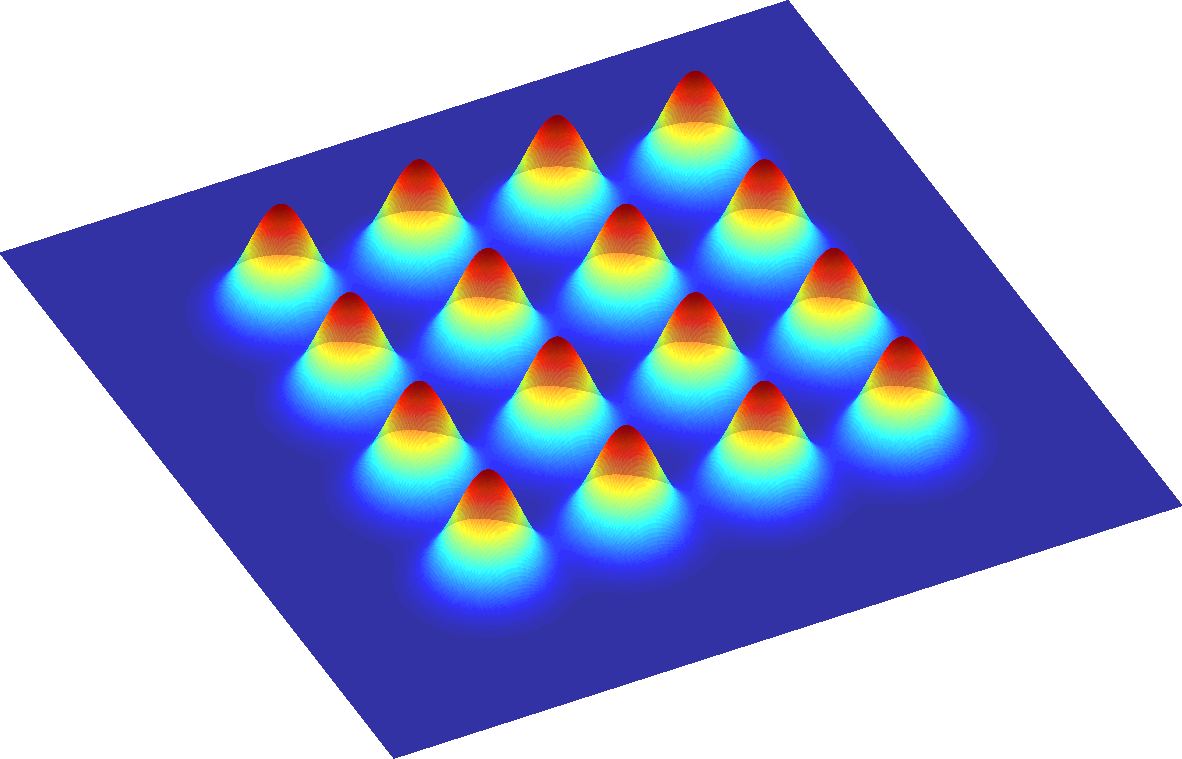
\includegraphics[width=\textwidth]{img/cellLayoutSquare.png}
        \caption{}
        \label{fig:cellLayoutSquare}
    \end{subfigure}
	\begin{subfigure}[t]{0.49\textwidth}
        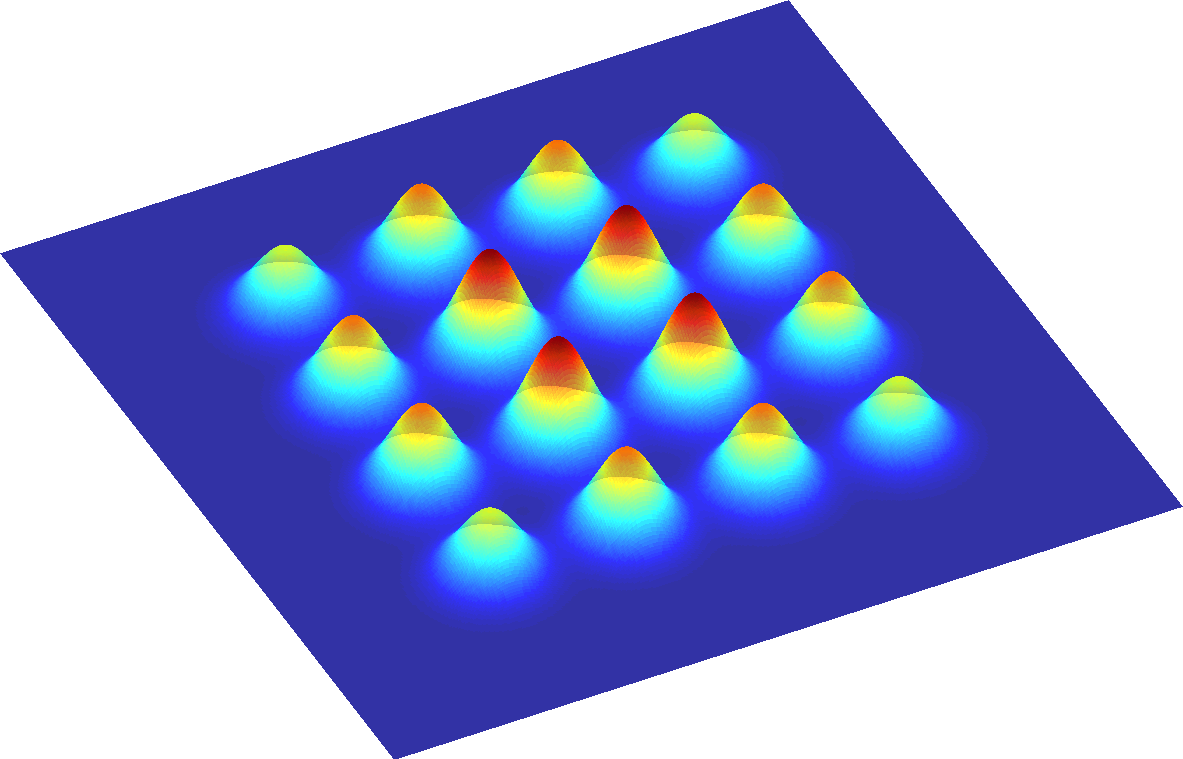
\includegraphics[width=\textwidth]{img/cellLayoutSquareCenter.png}
        \caption{}
        \label{fig:cellLayoutSquareCenter}
    \end{subfigure}
	\begin{subfigure}[t]{0.49\textwidth}
        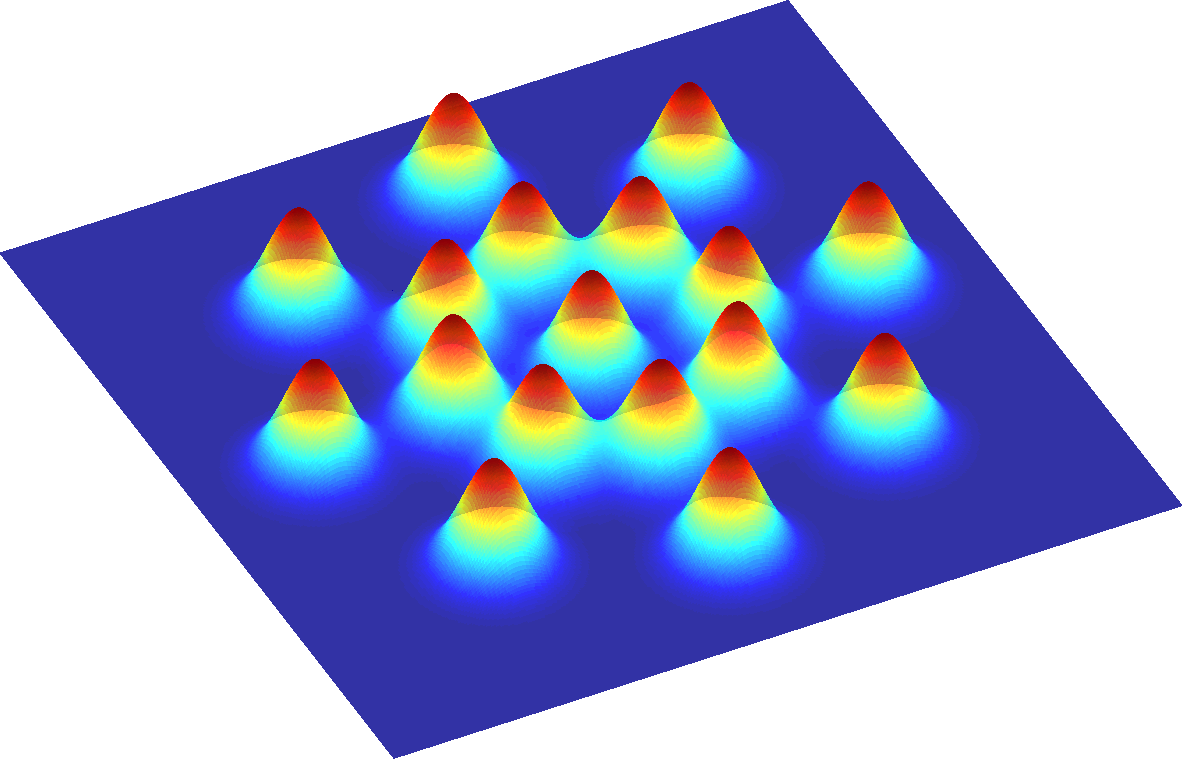
\includegraphics[width=\textwidth]{img/cellLayoutPolar.png}
        \caption{}
        \label{fig:cellLayoutPolar}
    \end{subfigure}
	\begin{subfigure}[t]{0.49\textwidth}
        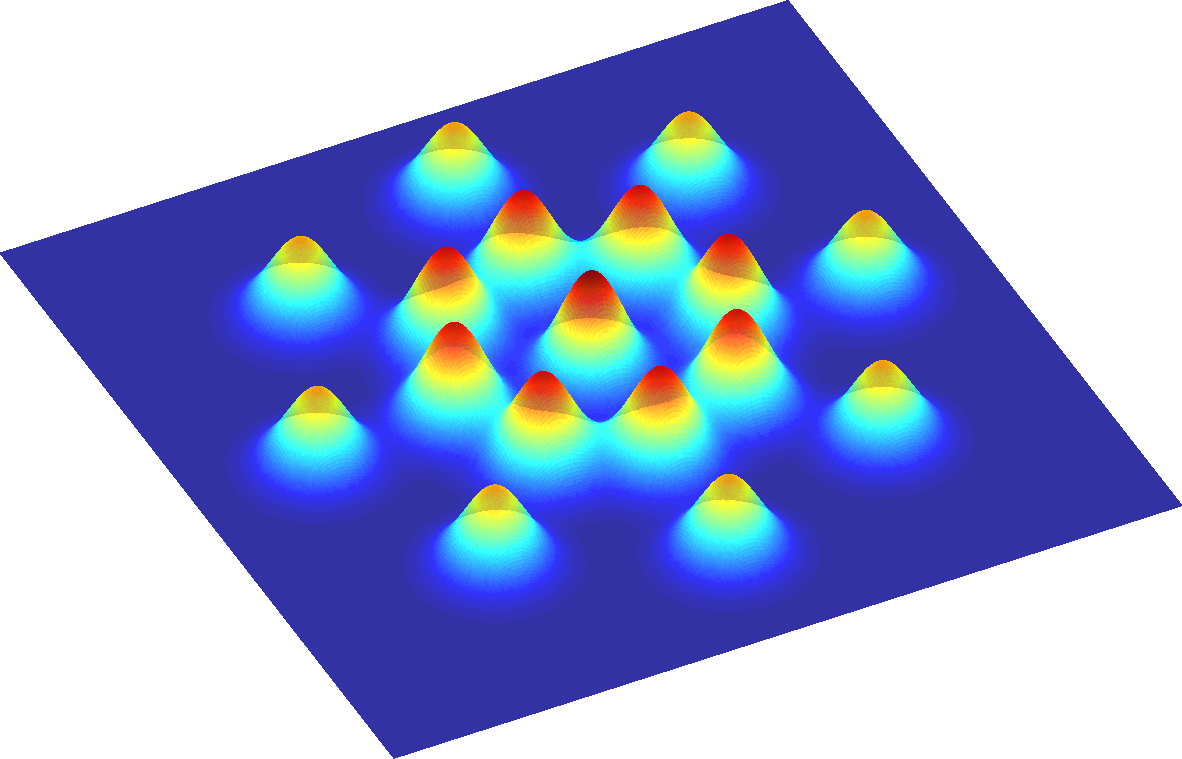
\includegraphics[width=\textwidth]{img/cellLayoutPolarCenter.png}
        \caption{}
        \label{fig:cellLayoutPolarCenter}
    \end{subfigure}
	\begin{subfigure}[t]{0.49\textwidth}
        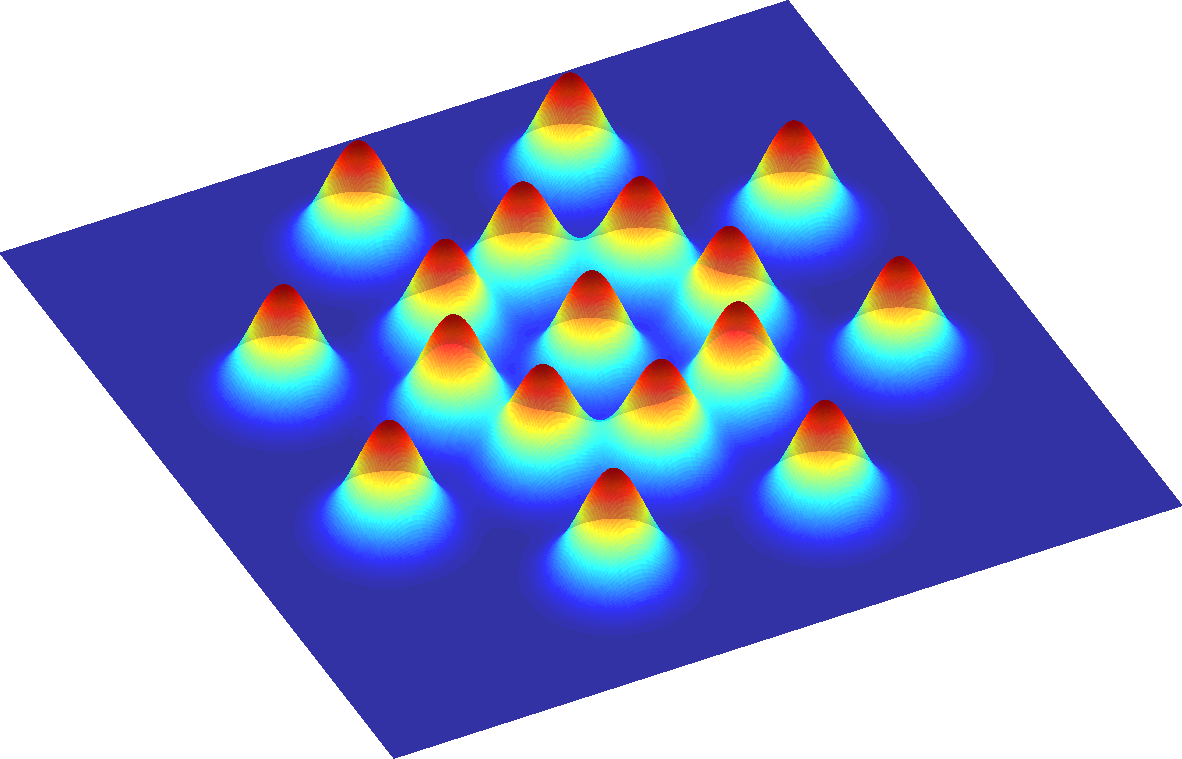
\includegraphics[width=\textwidth]{img/cellLayoutConcentricPolar.png}
        \caption{}
        \label{fig:cellLayoutConcentricPolar}
    \end{subfigure}
	\begin{subfigure}[t]{0.49\textwidth}
        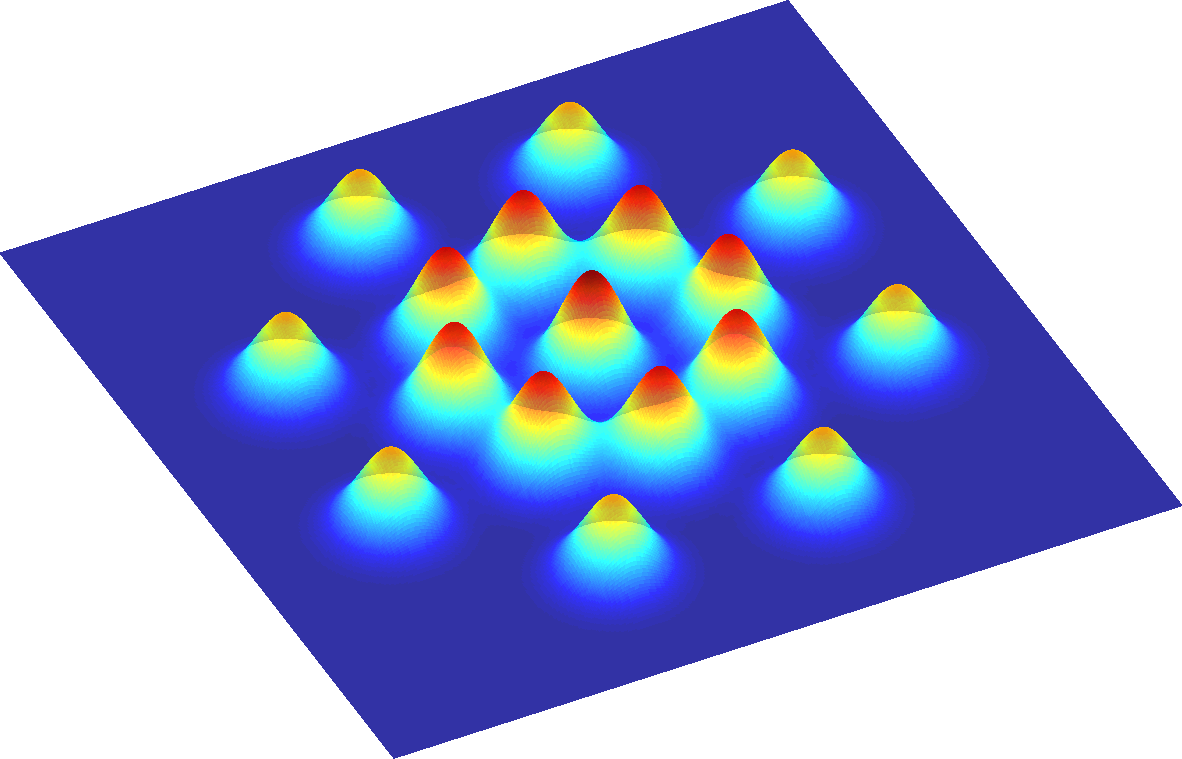
\includegraphics[width=\textwidth]{img/cellLayoutConcentricPolarCenter.png}
        \caption{}
        \label{fig:cellLayoutConcentricPolarCenter}
    \end{subfigure}
    \caption{}
\end{figure}
%
\begin{figure}[H]
    \centering
    \begin{subfigure}[t]{0.49\textwidth}
        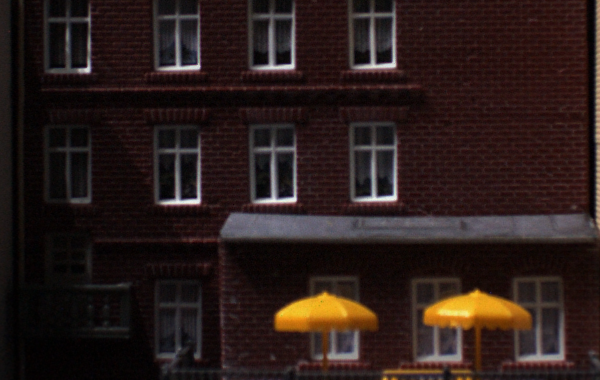
\includegraphics[width=\textwidth]{img/pixelNormalizationExample1.png}
        \caption{}
        \label{fig:pixelNormalizationExample1}
    \end{subfigure}
    \begin{subfigure}[t]{0.49\textwidth}
        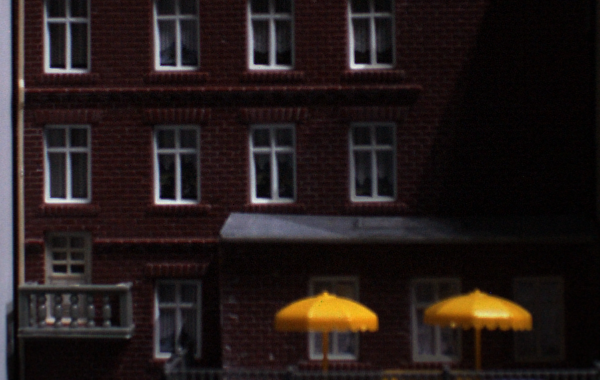
\includegraphics[width=\textwidth]{img/pixelNormalizationExample2.png}
        \caption{}
        \label{fig:pixelNormalizationExample2}
    \end{subfigure}
    \begin{subfigure}[t]{0.49\textwidth}
        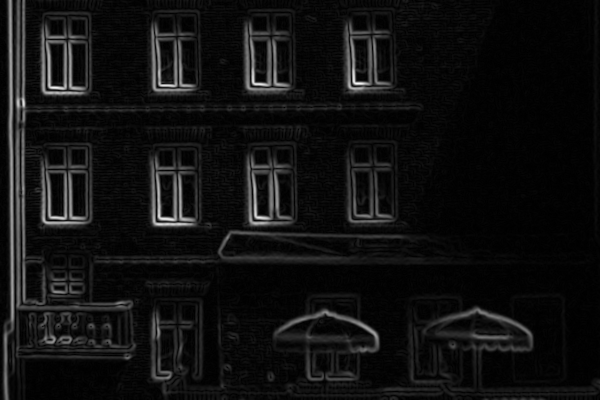
\includegraphics[width=\textwidth]{img/pixelNormalizationExample3.png}
        \caption{}
        \label{fig:pixelNormalizationExample3}
    \end{subfigure}
    \begin{subfigure}[t]{0.49\textwidth}
        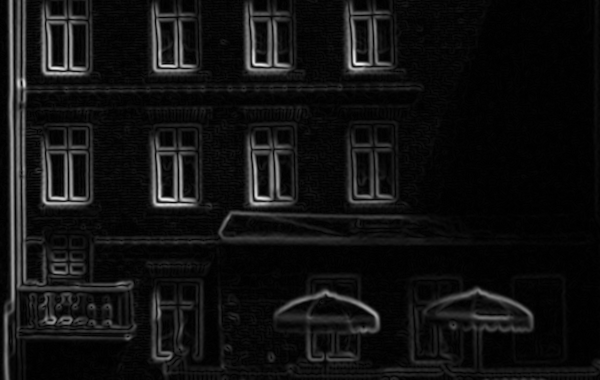
\includegraphics[width=\textwidth]{img/pixelNormalizationExample4.png}
        \caption{}
        \label{fig:pixelNormalizationExample4}
    \end{subfigure}
    \begin{subfigure}[t]{0.49\textwidth}
        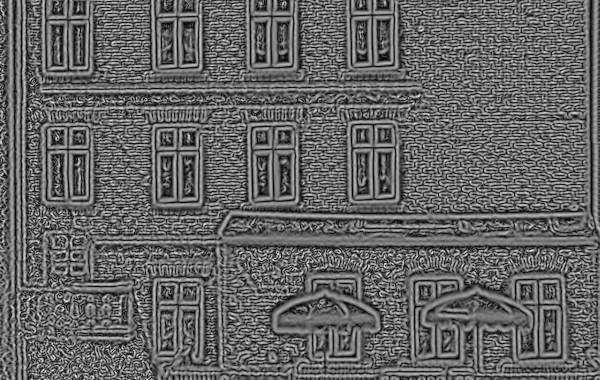
\includegraphics[width=\textwidth]{img/pixelNormalizationExample5.png}
        \caption{}
        \label{fig:pixelNormalizationExample5}
    \end{subfigure}
    \begin{subfigure}[t]{0.49\textwidth}
        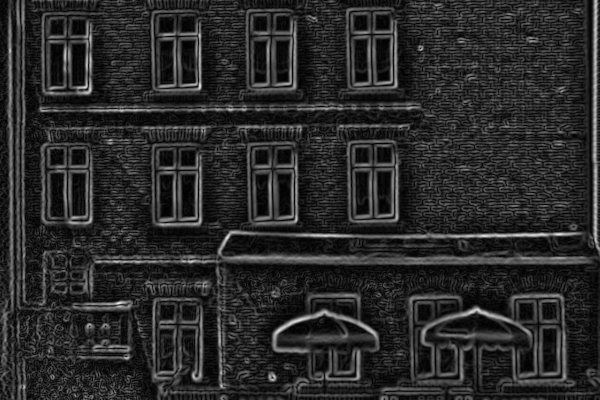
\includegraphics[width=\textwidth]{img/pixelNormalizationExample6.png}
        \caption{}
        \label{fig:pixelNormalizationExample6}
    \end{subfigure}
    \begin{subfigure}[t]{0.49\textwidth}
        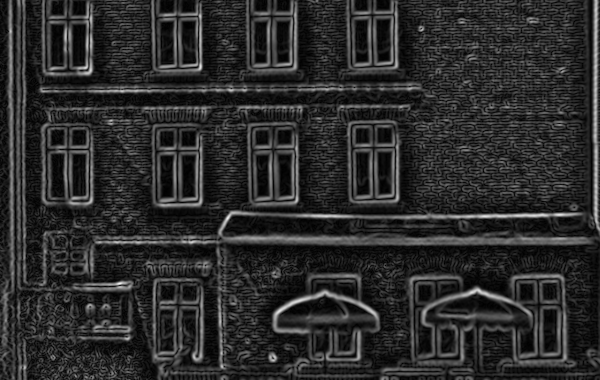
\includegraphics[width=\textwidth]{img/pixelNormalizationExample7.png}
        \caption{}
        \label{fig:pixelNormalizationExample7}
    \end{subfigure}
    \begin{subfigure}[t]{0.49\textwidth}
        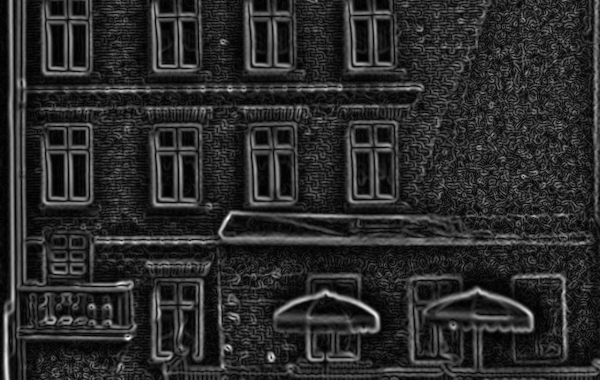
\includegraphics[width=\textwidth]{img/pixelNormalizationExample8.png}
        \caption{}
        \label{fig:pixelNormalizationExample8}
    \end{subfigure}
    \caption{Images \subref{fig:pixelNormalizationExample1} and \subref{fig:pixelNormalizationExample2} show cut-outs of an image with leftmost and rightmost artificial lighting, respectively. Images \subref{fig:pixelNormalizationExample3} and \subref{fig:pixelNormalizationExample4} show gradient magnitudes of these images. Images \subref{fig:pixelNormalizationExample5} and \subref{fig:pixelNormalizationExample6} show pixel normalized magnitudes for $\sigma_\text{norm} = 2$. Images \subref{fig:pixelNormalizationExample7} and \subref{fig:pixelNormalizationExample8} show pixel normalized magnitudes for $\sigma_\text{norm} = 10$.}
    \label{fig:pixelNormalizationExample}
\end{figure}
%
\subsection{Histogram normalization}

- No cell normalization -> Center (cell)

0. Center (pixels) -> no normalization
1. Center (pixels) -> cell normalization
2. Center (pixels) -> Cell normalization -> Center (cell)
3. Cell normalization -> Center (cell)

Center (cell)



\section{Performance evaluation}
%
%\section{Sliding window}
%
%\section{Spatial pooling schemes}
%
%\section{Normalization (local)}
%
%\section{Rotational invariance}
%
%\section{Histograms}
%
%\section{PCA}
%
%\section{Gradient orientation}
%
%\section{$k$-Jets}
%
%\section{Shape index}

\subbibliography

\end{document}
